\documentclass[11pt]{article}
\usepackage{geometry}                % See geometry.pdf to learn the layout options. There are lots.
\geometry{letterpaper}                   % ... or a4paper or a5paper or ... 
%\geometry{landscape}                % Activate for for rotated page geometry
%\usepackage[parfill]{parskip}    % Activate to begin paragraphs with an empty line rather than an indent
\usepackage{graphicx}
\usepackage{amssymb}
\usepackage{epstopdf}
\usepackage{amsmath}
\usepackage{xcolor}
\usepackage[round]{natbib}
\usepackage{tabularx}
\DeclareGraphicsRule{.tif}{png}{.png}{`convert #1 `dirname #1`/`basename #1 .tif`.png}
\linespread{1.5}


\title{Climate risk management: Drought and rangeland livestock production in the American West
}
\author{Trisha Shrum, William Travis, Travis Williams, Evan Lih, and Maxwell Roland}
%\date{}                                           % Activate to display a given date or no date

\begin{document}



\maketitle

\section{Front Parking Lot}
\begin{itemize}
\item We said that our argument is that ranching can inform other aspects of climate risk, but we do not clearly make this argument. Even if we just set this up for future work to be done, we need to make this very clear.
\end{itemize}


\section{Introduction}
\textcolor{blue}{Livestock ranching on semi-arid rangelands involves some of most complex decision-making of any natural resource production and land use system.} Ranchers engage in continuous adjustments to weather, climate and range conditions that affect livestock production and respond to weather-sensitive swings in feed prices and cattle markets. Studies of rancher responses, especially to drought, can cast light on climate risk challenges in that industry and offer lessons for complex decision-making in other weather- and climate-sensitive sectors. Insights gleaned in this setting may improve our understanding of universal problems in decision-making under uncertainty.  %Revisit this paragraph after reorganizing the paper

This review examines the literature relevant to the choices that ranchers make in the face of drought; the goal is to extract findings that situate the range livestock system in the context of climate risk management \citep{Travis2014}. \textcolor{blue}{Our argument is that rangeland livestock producers have developed a complex suite of strategies and tactics that can inform other aspects of climate risk---such as the expected utility of sequential decisions under uncertainty, value of additional information such as drought monitoring and forecasting, and risk aversion and risk transference tools like insurance.} The literature on this topic is a mixture of research articles and extensive gray literature such as agricultural extension service publications and research station reports. The review is also meant to provide the basis for new efforts to model and prescribe livestock producer response to drought, especially in the context of rainfall index insurance. %Make a case for how we are adding to the literature. Why should climate risk management folks care about ranching? 

\section{The Climate Problem in Ranching}
\textcolor{blue}{Pastoralism has long been studied as a dynamic socio-ecological system \citep{Galaty1990}, and as an exemplar of human adaptation to environmental variability.} In their review of global pastoralism studies, \citet{Reid2014} identified a set of key insights into how pastoralists use movement, collaboration, market hedging, and other adaptive mechanisms to thrive despite the large natural variability common in semi-arid rangelands, where “vegetation and water resources are usually ephemeral in time and patchy in space” (p. 219). They noted that flexibility and adaptability, hallmarks of the range livestock production, are necessitated by the uncertainty inherent in rangelands, which exhibit nonlinear dynamics, difficult-to-identify tipping points, and responses to different grazing pressures. For example, climate variation can either amplify or attenuate the effect of grazing pressure in determining rangeland ecosystem behavior \citep{Briske2005, Ellis1988, Wehrden2012}. Livestock production in the western U.S., regionally referred to as ranching, is a form of pastoralism, an adaptable natural resource production system exhibiting complex interactions among weather/climate, range condition, cattle and land management, markets, socioeconomics, and policy. 

\textcolor{blue}{Drought is the key natural hazard in western U.S. range livestock production.} 
%Numbers on how drought affects producers. 
Drought reduces the forage supply on which cattle weight gain and revenues depend, and can have macro impacts on cattle markets. For example, if widespread drought causes many producers to cull their herds simultaneously, then market prices can drop significantly \citep{Scasta2016a}.  Drought may also raise the cost of adaptation measures, through increased demand for rental pasture and supplemental feed. These price increases put further financial strain on producers that need to undertake drought adaptation in order to hold on to their herds through periods of low forage growth. When the cost of feed and rental pasture is too great, ranchers may sell cattle they cannot afford to feed resulting in widespread herd reductions and a cattle market in oversupply, which leads to reduced prices received by producers. Selling early to avoid this crunch comes at a cost: ranchers secure a better price per pound, but sell smaller cattle than if they kept them on the range or on supplemental feed and sold them later in the season. Once prices drop, producers have an incentive to try to hold on to their herd to wait out the drought and the depressed market, but this incurs other costs. They either pay for costly adaptation methods such as buying hay and renting pasture, or leave their herds on a drought-compromised range, which reduces livestock performance. If cattle are left to graze beyond what is optimal for the rangeland eco-hydrology, then the damages may affect long-term forage potential and future profitability. These many decisions and their outcomes are part of a complex, sequential chain of climate risk management on the ranch.

\section{The Drought-Ranching Connection: From the atmosphere to the sale barn}
\textcolor{blue}{This review is organized by the links and sequential decisions in the range livestock production system, starting with drought and working through cow-calf operating decisions to final marketing.} Our archetype ranch is a cow-calf enterprise, common in the American West, that maintains a ``mother herd'' and raises calves, born in the spring each year to be sold at auction typically in the fall \citep{Tess2000}.

Precipitation, forage growth, calving rate, weight gain, and sale price are critical variables in the range livestock production cycle and are among the variables commonly found in ranch simulation models and management spreadsheets. In addition to a linear flow from one factor to the next outcome (Fig. \ref{rainfall_to_marketing}), many of these variables interact with other factors in a complex manner. For example, market prices are affected by large-scale climate conditions through the climate-driven behavior of producers. \textcolor{blue}{The foundation and starting point is the interaction of climate and range: in the semi-arid rangelands of interest here, more precipitation typically yields more forage, which generally translates into larger cattle weight gain (or less supplemental feed to achieve a target weight).}

\begin{figure}
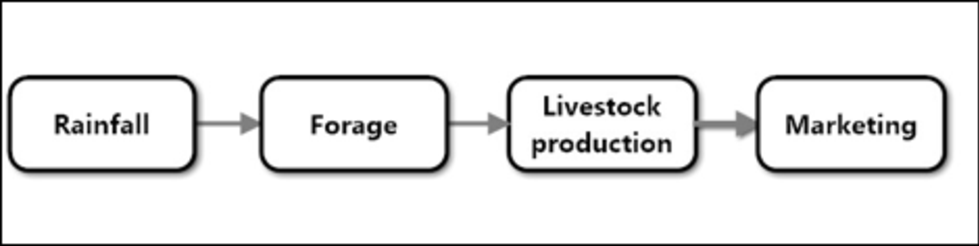
\includegraphics[scale=1]{rainfall_to_marketing}
\label{rainfall_to_marketing}
\caption{A simple schematic of the linear flow from rainfall to cattle sales.}
\end{figure}
 
\subsection{From Rainfall to Forage}
\textcolor{blue}{The critical first link in climate and ranching is between precipitation and forage production \citep{Cable2009}}. This relationship can be evaluated in two frameworks: short-term swings in forage production due to seasonal and intra-seasonal variation, especially drought, and long-term range production that sets the land's carrying capacity or sustainable stocking rate.

\subsubsection{Short-term Rainfall: Inter-annual and Intra-annual Variation}
\textcolor{blue}{An abundance of literature documents a positive correlation between precipitation and forage growth in semi-arid climates like the American West \citep{Yang2008, Cable1975, Houerou1977}.} The relatively straightforward relationship between average monthly precipitation and forage growth potential in the western U.S. was used by the Agricultural Research Service to create ``Drought Calculator'' spreadsheet decision tools to help ranchers and range managers predict forage reductions due to drought, based on observed monthly precipitation \citep{Dunn2013b}. In calibrating the drought calculator with site data on precipitation and forage, Dunn and colleagues account for 83\% of the variation in forage growth with monthly precipitation. 

\textcolor{blue}{Similar work supports this pattern of more precipitation leading to more forage, though the optimal temporal pattern of precipitation varies for different regions.} For example, in North Dakota, June is the key month for precipitation that yields forage growth \citep{Dunn2013b}. Rainfall earlier in the growing season is important further south: \citet{Smith2007} and Dunn et al. note that for most of Wyoming middle-elevation ranges, April precipitation is key to establishing total and peak standing forage. 

\textcolor{blue}{These intra-seasonal weights on forage production define key decision points.} For example, for middle-elevation ranges in Wyoming, if there is a precipitation deficit by the end of April, then it is unlikely that precipitation in later months will be able to fill the gap. This means that with an early deficit, drought management strategies should be decided upon by the end of April \citep{Smith2007}.  While the temporal effect of precipitation on forage varies across rangeland geographies, key periods in the Great Plains and Rocky Mountains, the region of interest for this review, tend to be spring and fall (both Dunn et al., and McCuistion et al. used climate data only for the spring and fall seasons). Winter and spring precipitation sets the basis for the initial spring growth, commonly known as the ``green-up'' of western ranges. Summer precipitation, which typically exhibits high variance in these regions, can add forage up to a point at which grasses mature and the correlation falls off. Fall precipitation affects cool season growth as well as over-winter forage conditions.

\textcolor{blue}{It is not only the quantity of forage that matters for cattle growth, but also the nutritive quality.} Forage nutritive quality is affected by, but not as tightly correlated with, rainfall. \citet{McCuistion2014a} tested the relationships among precipitation, season, temperature and forage nutritive quality, indicated by the amount of acid detergent and crude protein in the forage, two variables important to overall livestock health. Crude protein is the primary nutrient that livestock derive from forage, while acid detergent fiber (ADF) is the indigestible part of the forage – namely cellulose and lignin. They found that average monthly precipitation was only able to explain 37\% of the variation in forage nutritive quality \citep{McCuistion2014a}. With temperature and monthly precipitation included, the regression model accounted for up to 73\% of the ``variation for [crude protein] and ADF'' during the fall and spring seasons. The combined importance of precipitation and temperature points towards a clear role for climate risk, especially as both precipitation and temperature patterns change over time. However, it is important to note that temperature alone cannot account for increases or decreases in forage nutritive quality, as season and precipitation also play a large role in determine nutritive quality. 

\textcolor{blue}{Range simulation models dive deeper into the relationship between climate factors and forage by exploring ecological interactions of soil and plant life.} These models are built to explore the interplay between rangeland grazing and ecological responses; they are not generally meant to inform ranching decisions. We do not review them in detail here, but several links in such models emulate the chain of effects and decisions we address; a range process model may be a logical module of more complex range/ranch decision model. Table \ref{range_models} provide brief summaries of key rangeland models. %Why does this say 3.1 and not 1?

\begin{table}[htb!]
\begin{tabularx}{\textwidth}{|l|X|}
\hline
Model & Description \\
\hline
Century & The Century 5.0 Model is designed to simulate various nutrient cycles in four different plant-soil environments: grassland, forest, agricultural crop, and savannah systems. The Century model is primarily used for timescales of centuries to millennia but has recently added a daily time-step version, called DayCent5. DayCent5 includes trace gas and soil temperature sub-models \citep{Cerri2004}. \\
\hline
Phygrow & Phygrow (Phytograss Growth Model) –Developed by Texas A\& M. Primarily models forage consumption, above ground shrub/herb growth, and hydrologic processes. Determines how animal populations, weather, and varying landscapes affect forage production. Phygrow is unique in that it presents near instantaneous assessment for present and future forage conditions \citep{Souza2001}. \\
\hline
APEX (part of EPIC) & Agricultural Policy/Environmental eXtender Model. A Watershed Simulation Model created by Texas A\& M AgriLife Research. APEX’s purpose is to evaluate different land management strategies, while considering variables such as (but not limited to) soil quality, sustainability, economics, and plant competition. \\
\hline
\end{tabularx} 
\label{range_models}
\caption{Major range simulation models}
\end{table}
\clearpage


%Possible summary paragraph for this section? Otherwise, this section is in good shape!
%Add reference to APEX entry

\subsubsection{Long-term Rainfall: Climate and Range Carrying Capacity}
\textcolor{blue}{Climate interacts with edaphic factors like soil and plant community to determine the long-term productivity of rangelands \citep{Holechek2010}.} In terms of livestock production, the biomass production rate is translated into a ``stocking rate'' (i.e. carrying capacity), a quantity that expresses the basic productivity of the land via some quantity of forage it regularly produces and the number of livestock that forage can support.

\textcolor{blue}{The long-term carrying capacity of a ranch--the array of land (private and public) to which the producer has access--sets the limit for the size of the producer's herd.} 
%What do we mean by "think in terms of..."? Manage their herds? 
Carrying capacity may be expressed as a maximum herd size or as a rate, such as number of cattle per unit of land area or animal unit months (the forage needed to support an animal unit-- a cow and its unweaned calf-- for a month).

\textcolor{blue}{Determining sustainable stocking rates was one of the first big challenges of range science as it emerged in the middle of the 20th century} \citep{Bement1969, Harlan1958, Thomas2015, Paterson2012, Reppert1960, Fleischner1994}. Target stocking rates were needed to specify utilization of federal grazing permits and soon became the measure of productivity on private lands too. The basis for stocking rate calculations lies in the forage potential of a ranch under average conditions.
%What do we mean by grazing preferences? We don't define this at all... let's take it out unless there is a reason to keep it in
Forage is measured in mass per unit area, typically in pounds per acre. While ambiguities of definition remain, forage is usually interpreted as the edible biomass, thus excluding woody stems, produced over the growing season. 
%Add in a citation defining forage in our context from above(complete)
Cattle may not utilize all of this forage under normal circumstances; utilization rates reflect both grazing preferences of different animals as well as allowable or recommended harvest. \citep{Holechek1999, Redfearn2000}
%Might be a good time to define utilization rates with a reference

\citet{Holechek1988} developed a simplified set of equations to set the normal stocking rate for a ranch that is still in wide use today (Table \ref{stocking_rate}).
%What do we mean by allowable use? Define. 

%Go back to the paper and find what they were trying to say.
\textbf{Calculation of Total Usable Forage:}
\begin{equation}
F = P U A
\end{equation}

Forage production(lb/acre) X \% allowable use X area(acre) = Total forage(lb) available for grazing

\textbf{Calculation of Forage Demand:}
Weight of cows(lb) X daily forage intake (\% of body weight) X number of days pasture will be grazed = Forage demand (lb) per cow per year

\textbf{Calculation of Stocking Rate:}
Total usable forage (lb) / Forage Demand = Optimal stocking rate

Holechek’s calculation includes several simplifying assumptions: the range is in good condition, relatively flat, and is no more than two miles from a water source and the precipitation is normal. When computed based on 100\% utilization (meaning that livestock consume all the forage)
%Why are we assuming 100\% forage utilization when 30-50\% is recommended? Change numbers to 50%  utlilization and recompute.
 on a ranch of 1,000 acres comprised primarily of Blue Grama grass (a common species across the U.S. Great Plains), the formula produces a ranch suitable for 308 total cattle, or 3.25 acres per cow/calf unit. While Holechek’s calculations rely on the simplification of inputs, the study is still actively cited in 2017.

\textcolor{blue}{Stocking rate calculations are sensitive to cattle feed requirements, what Holechek called forage demand.} In the Great Plains and Rocky Mountain regions, a cow-calf pair typically needs 30-50 pounds of forage daily \citep{Cook2012}, or some 1-2,000 lbs. per month (also known as an “animal unit month, AUM).
%Is this typical? Does this differ from other regions? If so, why? Are these numbers typical for the US or just a region(what goes in to the forage demand, say it is above,below,average, compared to the average US needs. 
Stocking rates may range from as much as ten acres per animal in drier areas to as few as 2-3 in more productive areas. Single animals (e.g., a calf born the previous year and no longer paired with a cow) may require half the amount of rangeland \citep{Bement1969}. 


\textcolor{blue}{A paragraph about rangeland production rates.}
Because semi-arid rangelands produce somewhere between about 600 (in drier, hotter regions) and 2000 (in wetter, cooler regions) lbs/acre/year, each animal unit must have access to several acres. 

\textcolor{blue}{Moreover, grazing studies show that utilization rates (the proportion of total forage consumed) should be kept to around 35-50\% (especially in dry years) if the range is to remain healthy and productive over the long term \citep{Holechek1999}.}
% Especially in dry years: does this mean that they should eat a lower percentage of forage than is produced in a dry year? Or just that less forage is produced?
% What happens if you use more? 
% if you overgraze what happens to the landscape?(paragraph addition. conequences from ranchers perspective of over utilization and overgrazing)

\textcolor{blue}{A concluding paragraph about carrying capacity}


\subsection{From Forage to Cattle Production}
Mini-outline for the section:
\begin{itemize}
\item intro paragraph to note that cattle production (in pounds of calf) is determined by weaning percentage and calf weight gain. note that both are highly dependent on forage (and thus, rainfall)
\item Detail on weaning percentage
\item Detail on cattle weight gain
\end{itemize}

\textcolor{blue}{A paragraph on weaning percentage and forage}

\textcolor{blue}{Available forage is the key factor for cattle weight gain.} Numerous studies, algorithms and extension literature address this critical link. Harlan (1958) developed the first set of general curves for weight gain on different ranges at different grazing intensities. 
%This seems off topic:
In our study area feed requirements vary greatly depending on production strategy. 
%Is this repeated somewhere else?
The basic ranch in the West is a cow-calf operation that maintains a herd of mother cows who each produce one calf each spring and nurse them to near sale weights by the end of range growing season in October or November. Variations on this strategy include keeping some calves into a second year (i.e. yearlings or stockers) or buying yearlings to graze and then to be sold at their full adult weight the following season. Calves weigh 200-300 lbs. when they are born and 600-650 lbs. by when they are weaned from the mother cows. They are sometimes given time to gain additional weight after weaning through grazing or supplemental feed before being sold. From there, the literature on weight gain bifurcates into a quite large and varied body of “how to” and cattle management recommendations (e.g.,     ) and further research, including studies of weight gain under different grazing rotations, range sites, and weather and climate regimes (Grings et al. 1996) (Fang et al. 2014). 

\textcolor{blue}{Because forage production is mostly controlled by precipitation in the western ranges, some of the literature skips forage itself and simply correlates rainfall with weight gain.} In the cow-calf production system that is the focus of this study, research has found a positive correlation between precipitation and weaning weight---a calf’s weight when it is separated from its mother cow (John D. Scasta et al. 2015; Vantassell, Heitschmidt, and Conner 1987). Scasta et al. found that drought strongly impacts weaning weight: for each inch reduction of rainfall, weaning weight decreases by 7-14 pounds (John D. Scasta et al. 2015). 

\textcolor{blue}{This same correlation is also seen between precipitation and weaning weight.} 
%Make a distinction between weight gain and weaning weight. Why are we talking about these separately? Distinguish them and connect the discussion of one to the next
Many models use precipitation as part of their prediction of weaning weight, but do not directly use it as the sole predicting variable. (Gillard and Monypenny 1990). Vantassell et al. (1987) argued for a direct correlation between these two variables, stating that a calf’s rate of growth increases as precipitation increases with an asymptotic limit (Vantassell, Heitschmidt, and Conner 1987). Grings et al. assert that reduced precipitation also reduces forage nutritional value, and further affects calf weight gains (Grings et al. 2005). 

\subsection{From Production to Sales}
\textcolor{blue}{Ranchers seek to maximize their profits.}
%Bring in brief discussion of ranchers as profit-maximizers even when small scale ranchers tend to be family-owned and operated?
 To do so, they try to maximize revenues while minimizing the costs of production. Revenues depend on the number of cattle they sell, the quality and weight of those cattle, and the market price. 
 
\textcolor{blue}{Cattle prices have ranged around \$100-\$150 per hundred weight in recent years (Figure Xa).}  Prices vary seasonally; western cow-calf operations tend to market cattle in late fall of every year (e.g., Oct-Nov) in order to avoid the costs of over-wintering calves produced that spring. Because of the popularity of this production strategy, cattle supply tends to be high in the fall and prices decrease as a result (Holechek 1996; Holechek, Hawkes, and Darden 1994) (Brooks 2015). Different weight classes experience different price patterns (Figure Xb), but most show the fall slump. 

\textcolor{blue}{Some ranchers attempt to avoid the fall price by holding, and feeding, calves over-winter to become ``yearlings'' that can be sold anytime in their second year depending on sale and feed prices and available forage (xxxxx). Others take on ``stockers,'' typically another rancher’s calves or yearlings that can gain weight on the ranch given sufficient forage.} 
%Awkward/imprecise wording. Consider discussing the decision under uncertainty. Expected profits given uncertainty about rainfall and price. Also discuss how this can be a hedging mechanism.
The calculation here is whether stocker weight gain will pay off given additional costs, forage consumption, and off-cycle market prices.  
Because they can typically be profitable to sell at any time,
%How are they profitable at any time?
 yearlings and stockers are also seen as an adaptation to variable forage production; the drought adjustment literature recommends some inventory of cattle that can be sold at early signs of drought (xxx).

\begin{figure}
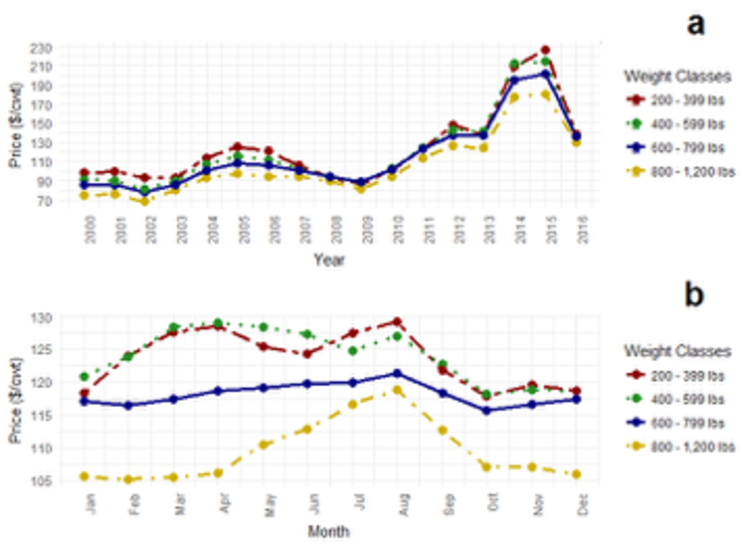
\includegraphics[scale=1]{prices}
\label{prices}
\caption{a: Average yearly sale price as dollars per hundred-weight for four weight ranges at U.S. cattle auctions from 2000 to 2016. b: Average monthly sale price as dollars per hundred-weight for four weight ranges at U.S. cattle auctions from 2000 to 2016. Source: The USDA Agricultural Marketing Service (https://www.ams.usda.gov/market-news/custom-reports)}
\end{figure}

\textcolor{blue}{Inter-annual price variation includes a well-known inventory and price swing called the ``cattle cycle'' (Crespi, Xia, and Jones 2010; Ritten, Frasier, et al. 2010), a form of a business cycle unique to the cattle market.}
%What is the cattle cycle?
The cattle cycle is associated with both the life-cycle of cattle herds and multi-year lags in response to forage availability, feed prices, and market signals (Norton 2005).
% I don't really understand what they are saying here... multi-year lags?
Drought is known to cause ranchers to cull their herds (to match reduced land carrying capacity as described earlier), and widespread drought increases the supply of cattle to the market, which depresses prices and exacerbates the cattle cycle. The 2012-2013 drought that affected much of the American Southwest and was the most severe drought in the southern Plains since the 1930s (Hoerling et al. 2014), and caused a significant drop in the national cattle inventory. Rebuilding herds takes time, and may be delayed by continued drought or expectations about continuing drought. In this situation, ranchers without cost-effective drought alternatives are forced to sell into a depressed market. Those who can arrange for alternative feed or grazing, and thus hold on to the herd, may try to wait for prices to rebound. In fact, prices tend to rise above average levels after a drought when supply is low due to low regional and national inventories and higher demand as ranchers buy animals to rebuild their herds (Bastian et al. 2006).

\section{Drought Response on the Ranch}
\textcolor{blue}{Ranchers practice strategic and tactical climate risk management by choosing among a well-known set of drought responses} (Coppock 2011) (Ritten, Bastian, et al. 2010; J. Derek Scasta, Lalman, and Henderson 2016; Kachergis et al. 2014). While the roster of options is well-developed, the decision process in the face of uncertainty is complex and less well studied. As Ritten et al. noted, ranch decisions are “complicated by variable range forage production caused largely by stochastic precipitation, and such decisions must often be made before growing season precipitation is realized” (Ritten, Frasier, et al. 2010). Long- and short-term herd management decisions must be calibrated to changing expectations of near- and long-term forage, weighing likely outcomes both in terms of economic returns and range ecosystem conditions (Derner and Augustine 2016).

Each drought adaptation choice has implications for the ranch enterprise, as well as potentially lasting effects on range ecosystems. 
%What kind of implications?

\textcolor{blue}{In terms of decision theory, producers operate in two major realms: expected utility under uncertainty (especially about climate, range, and market conditions) and strategic or game behavior in terms of anticipating the behavior of other producers (whose choices affect cattle and feed prices) and the government (which can offer supports like subsidized feed or other drought emergency programs).} Producers navigate this complexity with a mixture of tradition, intuition, analysis, and external advice, mediated by their risk perception and risk aversion. 

The daunting drought decision challenge was made clear during the 2011-2012 drought that caused the largest sell-off of the nation’s cattle herd in history:

%Indent this:
\begin{quote}
A [Kansas rancher] sold 20 pairs of cows and calves a few weeks after drought had sucked his pastures dry and no rain was in the forecast. He sold 20 more pairs Friday. [The rancher] spent years meticulously breeding his cows to improve the genetics each generation, but with Kansas in one of the worst droughts in decades, he’s struggling to find enough grazing to feed 300 cows, plus their calves. He hopes to get by with selling only a quarter of his herd, but there are no guarantees with the drought expected to linger through October. (Hegeman 2012).
\end{quote}

The news article further reported on the large sell-off, bringing the national inventory to a 40-year low and depressing cattle prices. It also described the fraught cycle in which ranchers cull herds en masse to save their pastures, selling into flooded markets at low prices, and later are forced to buy replacement animals at higher prices. 

\textcolor{blue}{One ranching strategy to is buck the trend, which is illustrated in another quote: ``If you can figure out a way to hang on to them at a reasonable cost until the drought is over, it typically pays you pretty well.''} Holding on means finding alternative feed and/or pasturage. But the urge to hold on, even as drought worsens, is often cited as a cause of long-term rangeland degradation (Knutson and Haigh, 2013; National Drought Mitigation Center, 2011). Much of the drought advice provided to ranchers warns against that strategy and, instead, encourages flexible and dynamic adaptation (Derner and Augustine 2016), including reductions in herd size to meet changing range conditions. 

\textcolor{blue}{In the worst case, ranchers may find themselves degrading range productivity, buying expensive feed, renting pasturage at inflated prices and, finally, selling into a market flooded by other producers who are also culling their herds (Hegeman, 2012).} They then pay a premium to rebuild herds in the drought’s aftermath (Gee, 2015). In 2015, with the industry in recovery, the Wall Street Journal could still find aversion to climate risks, quoting a rancher who was waiting to expand his herd back to its pre-drought levels: ``I’m not willing to spend \$2,000 or \$2,500 for a bred heifer and not know if I can make a profit next year… I’m not sure the drought is over'' (Gee, 2015). It is no wonder that one set of guides to ranch-drought management is sprinkled with suggestions for maintaining mental and physical health, and family well-being, through such tough choices (Knutson and Haigh, 2013; National Drought Mitigation Center, 2011). 

Such loss scenarios only play out if, indeed, drought continues. \textcolor{blue}{Decision theory (as well as producers) recognizes that uncertainty about even near-term future conditions—Will the drought continue? Will it worsen?— means that it is only in hindsight, with knowledge that the drought did, indeed, continue and worsen, that early adaptive decisions might seem justified.} Such advice may neglect the logic of expected value and the decision-maker’s assessment now of how they will feel about their choices if eventually proved as having been unnecessary and costly.
%Revise this sentence with care to make sure we are clear what the logic of expected value would be
%Should we name regret theory as a possible contributor?
Absent skillful forecasts of drought conditions over future months and seasons, the producer who chooses no action in the early stages of drought may well be wise, especially since most dry spells do not become extreme droughts.  
%What is the current state of long term drought forecasts: Look at DRMS proposal

\textcolor{blue}{This risky decision setting invokes a ranching strategy observed by range economists for decades: conservative long-term stocking rates that provide a buffer to drought impacts but fail to capture higher productivity when conditions are good (see, for example, Stafford Smith, 1992; Torell et al., 2010).} This strategy is observed in other resource systems in which productivity varies and is difficult to predict and monitor, like fisheries (Coulthard, 2009) and dryland cropping (Farahani, Petersen, and Westfall 1998). Ranchers, however, can adjust many aspects of their herd and land use on short notice and at several points in the annual cycle; the challenge during drought years is to break tradition and make those hard choices (Derner and Augustine 2016). 
%Headline on why we should care
%Possible discussion of the potential productivity gains of using less conservative stocking and adapting to drought dynamically

%moved this into this section... revisit
\textcolor{blue}{The extension literature is replete with warnings that not adjusting operations during droughts will incur losses, but the losses are poorly specified.} 
%This has nothing to do with the section as named
More precisely, the literature tends to focus on costs of adjustments (e.g., purchasing extra feed) rather than on the losses that accrue due to drought when no adaptive actions are taken (e.g., reduced gross receipts due to marketing at lower weights). This may stem from a reasonable assumption that most ranchers take some action to mitigate the effects of drought on cattle weight gain, typically buying feed or renting extra pasture as suggested by Derner and Augustine (2016) and most of drought advice gray and published literature. Yet there is analytical value, especially in decision studies, in calculating a clear baseline loss. The potential impacts of doing nothing are often described thusly:

%Quote is way too long. What really matters from this quote?
\begin{quote}
Cattle producers have few options when faced with drought. Some choose to do nothing different. However, this option is most likely not desirable as the reduction in forage produced will likely not allow animals to gain as much weight as desired. A second problem with this option is the long-term effect of reduced native rangeland resilience. Range in poor health requires more time to recover following a drought. Overuse of range during drought can also provide an opportunity for invasive species. Weeds tend to outperform native plants during drought-stressed times. Therefore, a producer concerned with long-term rangeland health will choose to be proactive in the face of drought. (Ritten et al. 2011)
\end{quote}

\textcolor{blue}{Summary paragraph that sets up how decision theory comes in and how we can learn from these decisions to inform decision theory and other climate risk management scenarios.}

\subsection{Drought and Ranching: A Role for Decision and Risk Theory}
The core problem laid out above-- how best to manage livestock and land in shifting weather and market conditions-- has been extensively studied, and that economic and ecological analysis (    ) has been translated into a wealth of advisory literature (        ) and decision support tools (      ).  As with agricultural economics research more widely, concepts of risk and risk management entered the range economics literature in the 1960s (Committee on Economics of Range Use and Development, 1966). This interest led to efforts to find evidence of optimal decisions in ranch operations (e.g., Rodriguez and Taylor, 1988). A body of detailed analysis of ranch decision-making has thus accumulated (Carande et al., 1995; Ritten et al., 2010a; Ritten et al., 2010b), and results have pointed toward the value of dynamic decisions that are responsive to changing conditions, especially during droughts (Derner and Augustine 2016). \textcolor{blue}{This instilled a long-standing operational question about adapting ranching to weather and climate variability: whether in general it is better to face weather and forage variability by a static, conservative long-term stocking rate or it is better to vary herd size and deployment(wc) frequently to match climate and range conditions} (see, for example, Stafford Smith, 1992; Torell et al., 2010). Recent drought management strategy advice has shifted toward dynamic adaptation (Ritten et al. 2011; Schmidt 2007; Beutler 2006a), thus putting more emphasis on rapid response and informed decision-making, along with nimble financial management, a strategy presumably enabled by better monitoring, data, forecasts, and analytical capacity. 

%What do we have to learn from ranching? What new insights can we bring from ranching to decision theory or climate risk management? What new insights from climate risk management can we bring to ranching?


\subsection{Drought Management Options}
\textcolor{blue}{At the center of the ranch-drought decision problem is the choice of alternative responses and their expected outcomes.} Agricultural extension services, and drought management entities like the National Drought Mitigation Center (National Drought Mitigation Center 2013) provide planning and decision tools aimed at this crux. We canvassed this literature, including especially extension advice and similar prescriptive publications and bulletins, plus the peer-reviewed literature, to build a propositional inventory of drought adaptations on a western ranch. (Table X). 

TABLE X

%Rethink this paragraph. Perhaps make it coincide with the categories in the table
In the face of drought, and with planning in advance and information gathering, ranchers can, for example:
1) reduce cattle numbers progressively with increasing severity and duration of drought, which is why having established critical dates for enterprise decisions is essential; 2) add forage quickly through leasing land, purchasing feed or moving cattle to alternate locations where forage is available, perhaps in other states (as was the case with the recent Southern Plains drought as cattle moved to the Northern Plains states); and 3) substantially increase enterprise flexibility by splitting forage between cow-calf and yearling enterprises….(p. 214)

The main adjustment is to somehow reduce stocking, that is, take cattle off of the range. The extension literature also suggests selectively thinning a herd to suit the forage available, starting with older cows and those that are not pregnant (e.g., Paterson et al. 2012). Along with this first round of culling, Paterson and co-authors recommend weaning calves early to reduce the nutritional demand on lactating mother cows. Recommended stocking and utilization rates for drought conditions are much less well established than those for periods of normal rainfall. Hart and Carpenter (2005) estimate that across the Great Plains and Mountain West that the carrying capacity of the range during drought may be 50-70\% of that in a normal year. A simple rule of thumb for keeping range healthy through droughts is to “take half/leave half” of the forage that is available, meaning potentially quite significant reductions in use of rangeland. Beyond that, the guidance in the literature for drought stocking rates is general and appears more in agricultural extension material (Hart and Carpenter 1999; Paterson et al. 2012) rather than the peer-reviewed literature. The technical advice literature also focuses on a key response to drought-reduced forage: obtaining supplemental feed to make up for reduced forage (   ). Supplemental feed can bring cattle to desired market weights despite drought-reduced rangeland production, but it entails additional costs. 

\subsection{Information: Key to Drought Decision-Making}
%Define all acronyms when they are first introduced.
Outline for this section:
\begin{enumerate}
\item Establish/reiterate that early decisionmaking is the key to drought management, but note that drought early warning systems are limited.
\item Describe current DEW products. Possibly give each DEW its own paragraph. 
	\begin{itemize}
	\item What is the product? What is the main goal/audience/usage?
	\item How does it predict/monitor
	\item What are the limitations?
	\end{itemize}
\item Any new/upcoming developments? Suggestions for further research/utilization?
\item Summarize how well current DEWs meet rancher needs for drought management
\item Bring this back to drought risk management: how does this affect optimal decisionmaking and risk management?
\end{enumerate}

Derner and Augustine (2016) point out that drought risk management on the ranch requires producers to make decisions at critical points in time. As precipitation becomes more variable, the timing of decisions becomes even more important \cite{Derner2016}. However, a proactive approach to drought management requires proactive information.



\textcolor{blue}{Droughts are slow-onset extremes and their pervasive temporal and spatial dimensions distinguish them from most other weather hazards dealt with by weather warning systems.} Recent events in the U.S., including the intense, prolonged drought in 2012-13, showed the value of integrated drought information. 
However, drought early warning systems, like the NIDIS DEWS, are structured differently than other weather early warning systems, and generally do not use the terminology nor communications strategies associated with extreme weather advisories and warnings.
%How are they structured differently? Is this helpful? Harmful? How could they be structured better? 
Still, drought early warning systems do contain some of the same elements as other warning systems. 
%I don't know what this sentence means:
For example, in cases where drought declarations are made or where river and reservoir levels are monitored and projected into ways meant to convey future risk. 
%What's the conclusion?
The major conclusion is that, 

This is mainly due to limits on seasonal forecasting. 
%What is mainly due to these limits?
The severe drought in summer 2012 in the southern Great Plains was not hinted at even in the 30-day outlooks issued just a couple of months prior (Heorling et al., 2017). 
%Why was a 30 day outlook issued months prior? What is a 30-day outlook?
Thus, drought ``early warning systems'' are not classical warning systems, instead, they rely on close links between monitoring and decision-making to evoke effective, proactive responses. 
%I don't feel like I learned anything about drought warning systems. Revamp this entire section.

Currently in the U.S. drought ``early warning'' is not focused on prediction and warning, but instead stress monitoring, detection, and diagnosis, and the dissemination of that information through products like the USDM (Fig. X), outlooks, briefings, webinars, all meant to help resource managers make better decisions. 
%Early warning seems like a misnomer here, reconsider the term 
The monitoring and assessment capabilities are built on regional drought and related information resources, such as those from state, tribal and local government,  utilities, and stakeholder groups of all sorts, enhanced with NIDIS-specific and other national and regional inputs such as those from USDA, USGS, USACE, BuRec and other agencies. 
%What kind of resources?

The monitoring and diagnostic approach is extended to prediction per se through the application of  NOAA-NWS long-range (6-14 days) temperature and precipitation forecasts, and to 1-3 month outlooks via Climate Prediction Center (CPC) products (Fig. 3), often applied to precipitation, streamflow, and lake levels. Some DEWS attend to the Seasonal Drought Outlook (SDO)%\footnote{See: http://www.cpc.ncep.noaa.gov/products/expert_assessment/sdo_summary.php)}}.
 The SDO (Fig. 3)
%Where is this figure?
 is based on seasonal prediction and is framed in terms somewhat similar to early warning by mapping places of future drought development over a 90 day period. Other DEWS stress NOAA El Nino watch and advisory products when in effect., in regions where the signal of El Nino is strong and offers some insight into, say, the coming 9-month conditions. 
 %This sentence is very confusing. Come back and untangle it.

Seasonal forecasts, and specifically drought prediction, offer limited skill (Hoerling et al., 2014). Some ``predictions'' in the DEW sense derive mostly from extrapolation of current conditions. 
For example, streamflow forecasts in the West tend to depend on current snowpack. 
They are extrapolated by empirical and simulation models, and may be modified by seasonal forecast.
% "They are extrapolated" doesn't really make sense. The DEWs?
Another type of forecast can come from leading indicators of drought. Researchers are developing the Evaporative Demand Drought Index (EDDI) as a sensitive, leading indicator that senses drought in its early stages (McEvoy et al. 2016; Hobbins et al. 2016). 
Such monitoring and detection process
% processes?
 is extended via mostly extrapolation of leading indicators to future conditions (e.g., current snowpack is used to extrapolate future runoff), and it further extended to prediction per se through the application of NWS long-range (6-14 days) temperature and precipitation forecasts, and to monthly and longer outlooks via NWS climate prediction products.  
% Make a clear distinction between extrapolation and prediction. This is a focus of a lot of the framing. So what exactly does it mean? Why is this distinction important?
Perhaps the key development in DEWS is integration of information providers and users, and improved designation and collaboration with regional decision-makers whose systems can be affected by drought. 
% How is this developing? If this is key, let's discuss it further.

\section{Conclusions}
The key climate risk management challenge in ranching in the face of drought is making decisions in a timely manner while the slow-onset event unfolds. While forecast value studies may reveal the benefits of forecast accuracy and lead time, drought early warning is characterized more by monitoring and early detection rather than prediction per se, and a broader measure of the value of DEWS might be the decision analysis criterion called Value of Information (VOI) or Value of Additional Information (VAI). The key to both approaches is the expected value of decisions made on the information, sometimes compared to the cost of providing or obtaining the information, but typically compared to absence of information. VOI has been applied to judging the social value of earth sensing data from NASA (National Aeronautics and Space Administration, 2012), and is applied in many business decisions (Clemen and Reilly, 2013). An important aspect of VOI analysis is that it encompasses both improved information (e.g., better forecast, more accurate or highly resolved monitoring data, or new indicators meant to be sensitive to critical variables) as well as improved decision-making. Thus, properly done, VOI analysis is agnostic to, for example, whether better snowpack forecasts are more valuable than better snowpack monitoring in terms of, say, reservoir operations and water supply outcomes. 
Given the different natures of monitoring and forecasting, one science policy question for the future is what investments would pay off more in terms of mitigating drought impacts. All three parts of DEWS as we have framed them, presumably would benefit from improvements, but the relative return on investments may not be obvious and is itself an area for additional analysis. 


\newpage
\bibliography{projectrisk}
\bibliographystyle{plainnat}

\end{document}